
% The WMT Server design
% 6/5/2000 jhrg
%
% $Id$

\documentclass{article}
\usepackage{epsfig}
\usepackage{rotating}
\usepackage{subfigure}
\usepackage{xspace}
\usepackage{vcode}
%\usepackage{changebar}
%\usepackage{acronym}
%\usepackage{gloss}

% Note: to get the gloosary to work, run bibtex in the registry.gls.aux file,
% then latex registry, then bibtex *.gls, then latex. Also, make sure to set
% your BST and BIBINPUTS environment variables so that the BST and BIB files
% will be found.
%\makegloss

% Change paragraph typesetting; eliminate indenting and add more space between
% paragraphs. 2/15/2000 jhrg
\setlength{\parindent}{0em}     % Amount of indentation
\addtolength{\parskip}{1ex}     % Vertical separation

\newcommand{\Cpp}{{\rm {\small C}\raise.5ex\hbox{\footnotesize ++}}\xspace}
\newcommand{\DAP}{{\rm {\small DAP}\raise.5ex\hbox{\footnotesize ++}}\xspace}
\newcommand{\DASllc}{Data Access Software, {\footnotesize {\sc L.L.C.}}\xspace}

\begin{document}

\title{DODS OpenGIS World Map Gateway Design}
\author{James Gallagher\thanks{Data Access Software, jgallagher@gso.uri.edu}
        \and Dan Holloway\thanks{Data Access Software, dholloway@gso.uri.edu}}

\date{\today \\ $Revision$ }

%\bibliographystyle{plain}

\maketitle
\tableofcontents

\section{Introduction}

This document describes the design for the DODS-WMT Gateway, version
1.0. Because the server is a joint project between \DASllc (DAS) and Goddard
Space Flight Center (GSFC), this design focuses on the software built by DAS
and describes the interface between that software and the software developed
by GSFC.

The software written by DAS uses the DODS \Cpp \DAP library. The object
oriented design is presented here using diagrams written in UML.  However,
we've taken some liberties with the notion of a `class' in cases where
that simplifies the diagrams. In addition, the descriptions of the classes
presented here are minimal. This design describes, in most cases, the
interface between parts of the DODS-WMT Gateway and not how they are to be
implemented.

We use the word \emph{Gateway} rather than \emph{Server} to emphasize that
this software adapts the WMT protocol to am existing set of data servers
(DODS servers) and that the software relies on those servers to access data.

Everywhere in the text where we say \emph{the DODS-WMT Gateway} we mean
version 1.0 unless the text explicitly says otherwise.

Section~\ref{sec:components} describes the different software components that
implement the server. Section~\ref{sec:gateway} describes the classes which
comprise the components built by \DASllc and its interfaces to the parts of
the server built by GSFC.

In the text, brackets ([]) are used to indicate sections of the OpenGIS Web
Map Server Interface Implementation Specification, Revision
1.0.0\footnote{OpenGIS Project Document 00-028, Release Date: 19 April
  2000.}, that we often refer to as simply the \emph{WMT specification}.

\section{Components of the DODS-WMT Gateway}
\label{sec:components}

Figure~\ref{fig:component} shows the DODS-WMT Gateway, its components, and
how those interact with other software when the server is asked to handle a
request. A WMT client program sends a request using HTTP to the DODS-WMT
server. This request is actually initially handled by the WMT server's httpd
which uses the CGI 1.1 interface to pass parameters to the DODS-WMT
Gateway\footnote{For the rest of this paper, we assume that httpd's role is
  understood.}. Once the DODS-WMT Gateway gets the request parameters, it can
begin to answer the request.

If the client has made a Capabilities request then the DODS-WMT Gateway will
return a static XML document that can be read from the local host's file
system. In this case the DODS-WMT Gateway does not need to interact with a
DODS server.

If the client request is a Map request, the DODS-WMT Gateway must translate
the parameters of that request into a data request for the DODS server and
process the returned information to build a correct response for the client.

The 1.0.0 version of the WMT specification does not address selecting single
granules from data sets which are comprosed of many granules spread out in
space and/or time.\footnote{Terms such as \emph{data elements} and
  \emph{granules} are all loaded with multiple meanings. We are using the
  term \emph{granule} to mean a single file in a data set made up of many
  files.} We tested the WMT Gateway against such a dataset and developed one
solution for selecting granules in time using the WMT Vendor Specific
Parameters. The class CatalogURL, a specialization of DodsURL, implements
this feature (See Section~\ref{dodsurl}).

The optional FeatureInfo request will not be handled by the first version of
the DODS-WMT Gateway. However, the architecture described here is clearly
capable of supporting that request.

\begin{sidewaysfigure}
\begin{center}
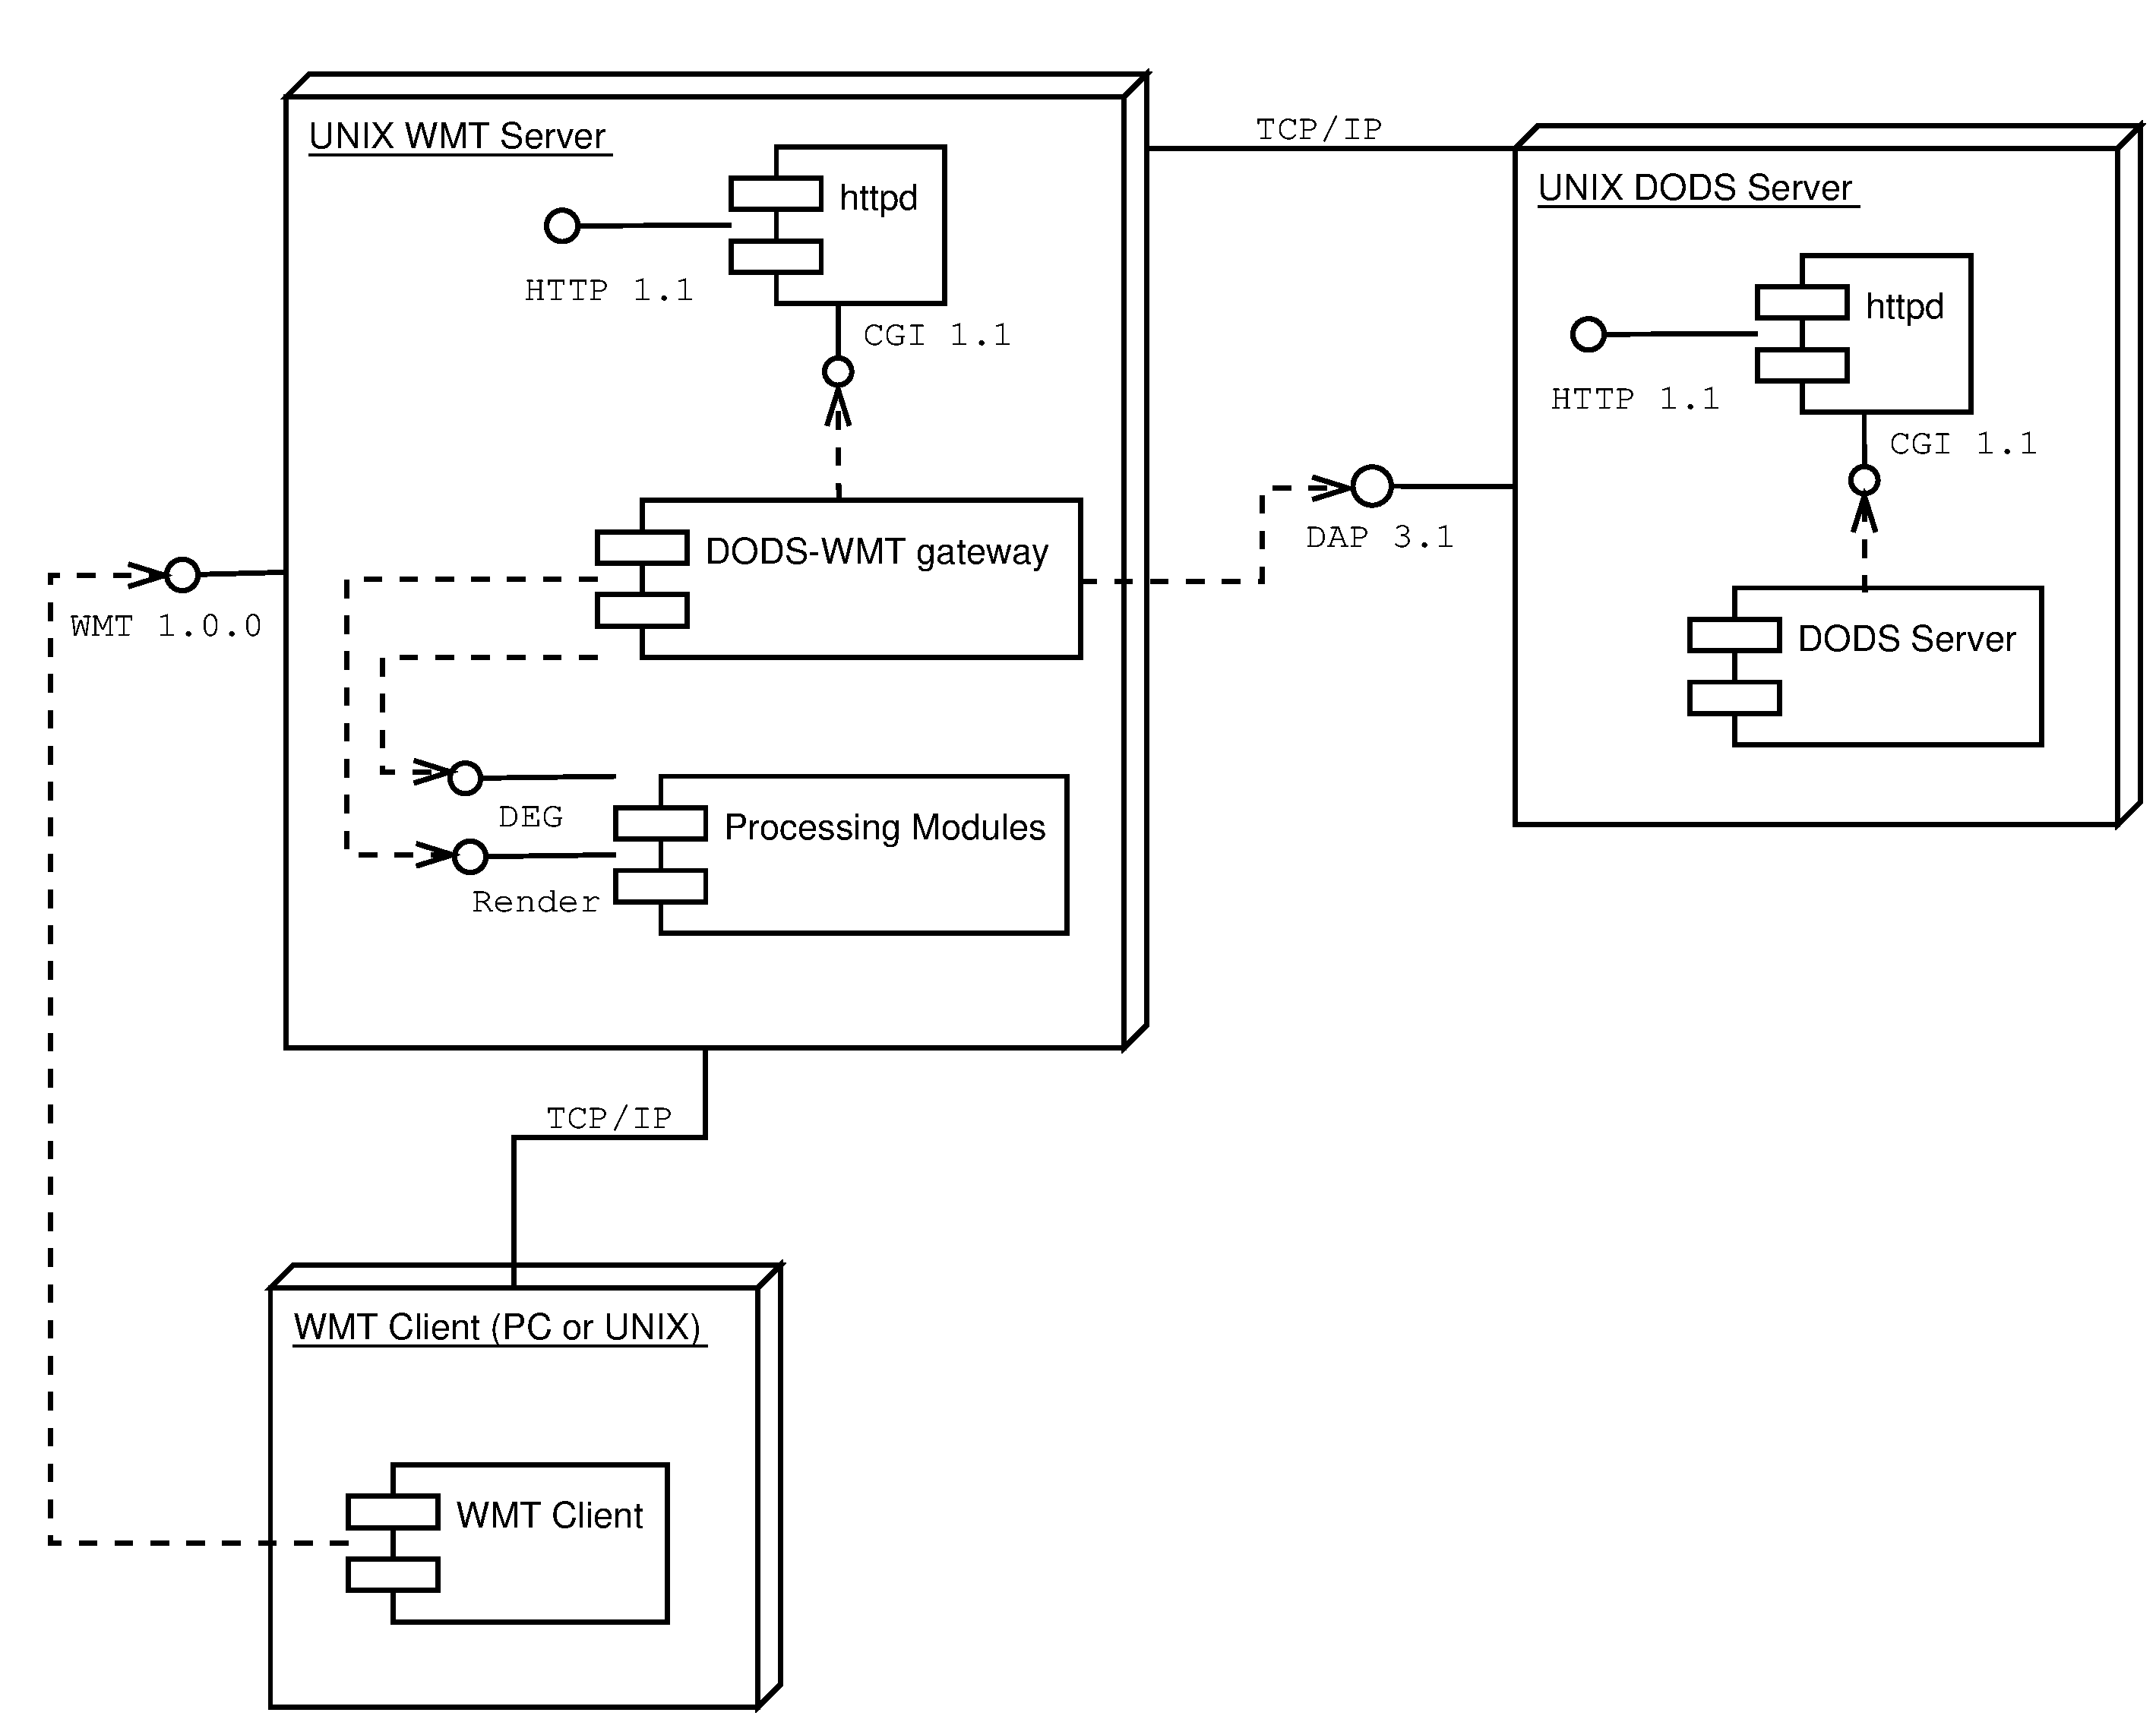
\epsfig{file=wmt-component.eps,width=8in}
\caption{A Combined Deployment and Component diagram for the DODS WMT Gateway.
  Only the DODS-WMT Gateway and Processing Modules components need to be
  built; the other components already exist.}
\label{fig:component}
\end{center}
\end{sidewaysfigure}

\section{Classes in the DODS-WMT Gateway}
\label{sec:gateway}

\begin{sidewaysfigure}
\begin{center}
\epsfig{file=wmt-class-v4.eps,width=8in}
\caption{A Class diagram for the DODS-WMT Gateway. This diagram specifies the
classes and their interfaces, not the absolute implementation.}
\label{fig:class-v4}
\end{center}
\end{sidewaysfigure}

The DODS-WMT Gateway may or may not be implemented formally as a \Cpp class.
However, it is simplest to think of it as a \Cpp class which has a main
method. This software, whether actually a collection of functions or a formal
class, will instantiate the other classes shown in Figure~\ref{fig:class-v4}
in response to a request.

In addition, the DODS-WMT Gateway software will contain the WMT specification
version number corresponding to the DODS-WMT Gateway's implementation. As the
DODS-WMT Gateway is updated to match revisions in the WMT specification, this
information will also be updated as described by section [6.1.3] of the WMT
specification. 

The DODS-WMT Gateway class uses several primary classes to respond to
a WMT client request.  These classes are used to represent the server's
capabilities, the client's request parameters, and provide mechanisms
for accessing DODS-served data and transforming it into the requested
WMT-compliant format.

In the following, see Figure~\ref{fig:class-v4}.

\subsection{Managing the request parameters}
\label{sec:request}
Requests may be presented using either HTTP's GET or POST mechanisms [6.2.5].
The MapRequest object will parse those parameters and record their contents.
MapRequest will provide accessor methods for each of the possible request
parameters. The MapRequest object will be used by the DODS-WMT Gateway as well
as other objects to access parameters passed to the server. The MapRequest
object must satisfy all of the requirements of section [6.2.5] of the WMT
specification.

\subsection{Version negotiation}
\label{sec:negotiation}
The Capabilities object will be responsible for satisfying the requirements of
sections [6.1.1] and [6.1.4] of the WMT specification. The actual process of
negotiation is straightforward.

\subsection{The Capabilities request}
\label{sec:capability}

% The interaction diagrams are wrong and, with the current organization of
% the software, will be too hard to draw. 10/20/2000 jhrg
%
% \begin{figure}
% \begin{center}
% 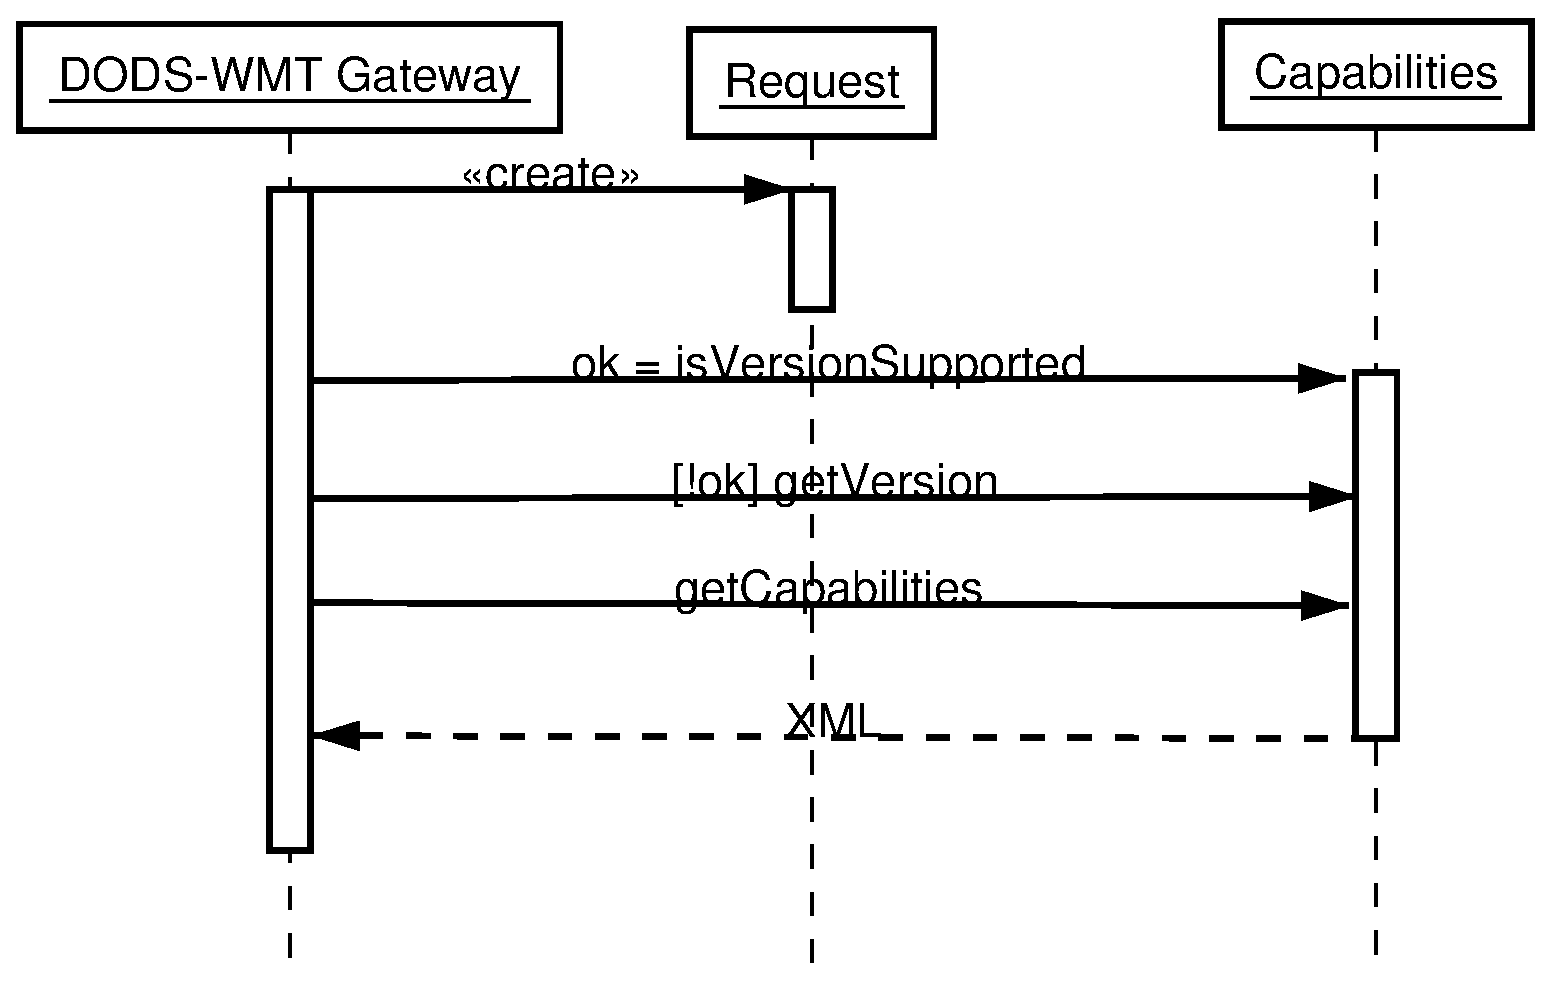
\epsfig{file=wmt-interaction-cap.eps,width=5in}
% \caption{A sequence diagram for the Capabilities Request.}
% \label{fig:interaction-cap}
% \end{center}
% \end{figure}

Version 1.0 of the DODS-WMT Gateway will respond to a Capabilities
request by returning a static XML document (see [6.2.7.1] of the 
WMT specification) to the client.  Rather than have the DODS-WMT 
Gateway object handle reading the XML document, the 
Capabilities class hides the actual process
used to generate the document so that we can easily extend its 
functionality to dynamically generate the XML response in the future.

The capabilities object must satisfy all of the requirements of section
[6.2.7] and the XML DTD contained in Annex A of the WMT specification.

In addition, the Capabilities object will have methods needed to access
information for version negotiation. The object will also serve as a way for
other objects to learn about the server. For example, it will provide a way
for other objects to find a DODS URL which corresponds to a particular Layer
value.

The Capabilities object will use a static table to map Layers to DODS URLs
for its own internal use. This will provide a simple way to accommodate new
DODS servers without changing the \Cpp software (i.e., the static table can be
updated using a text editor and will require no compilation, etc.).

% Figure~\ref{fig:interaction-cap} shows the objects involved in responding to
% a Capabilities request.

\subsection{The Map object}
\label{sec:map}

% \begin{sidewaysfigure}
% \begin{center}
% 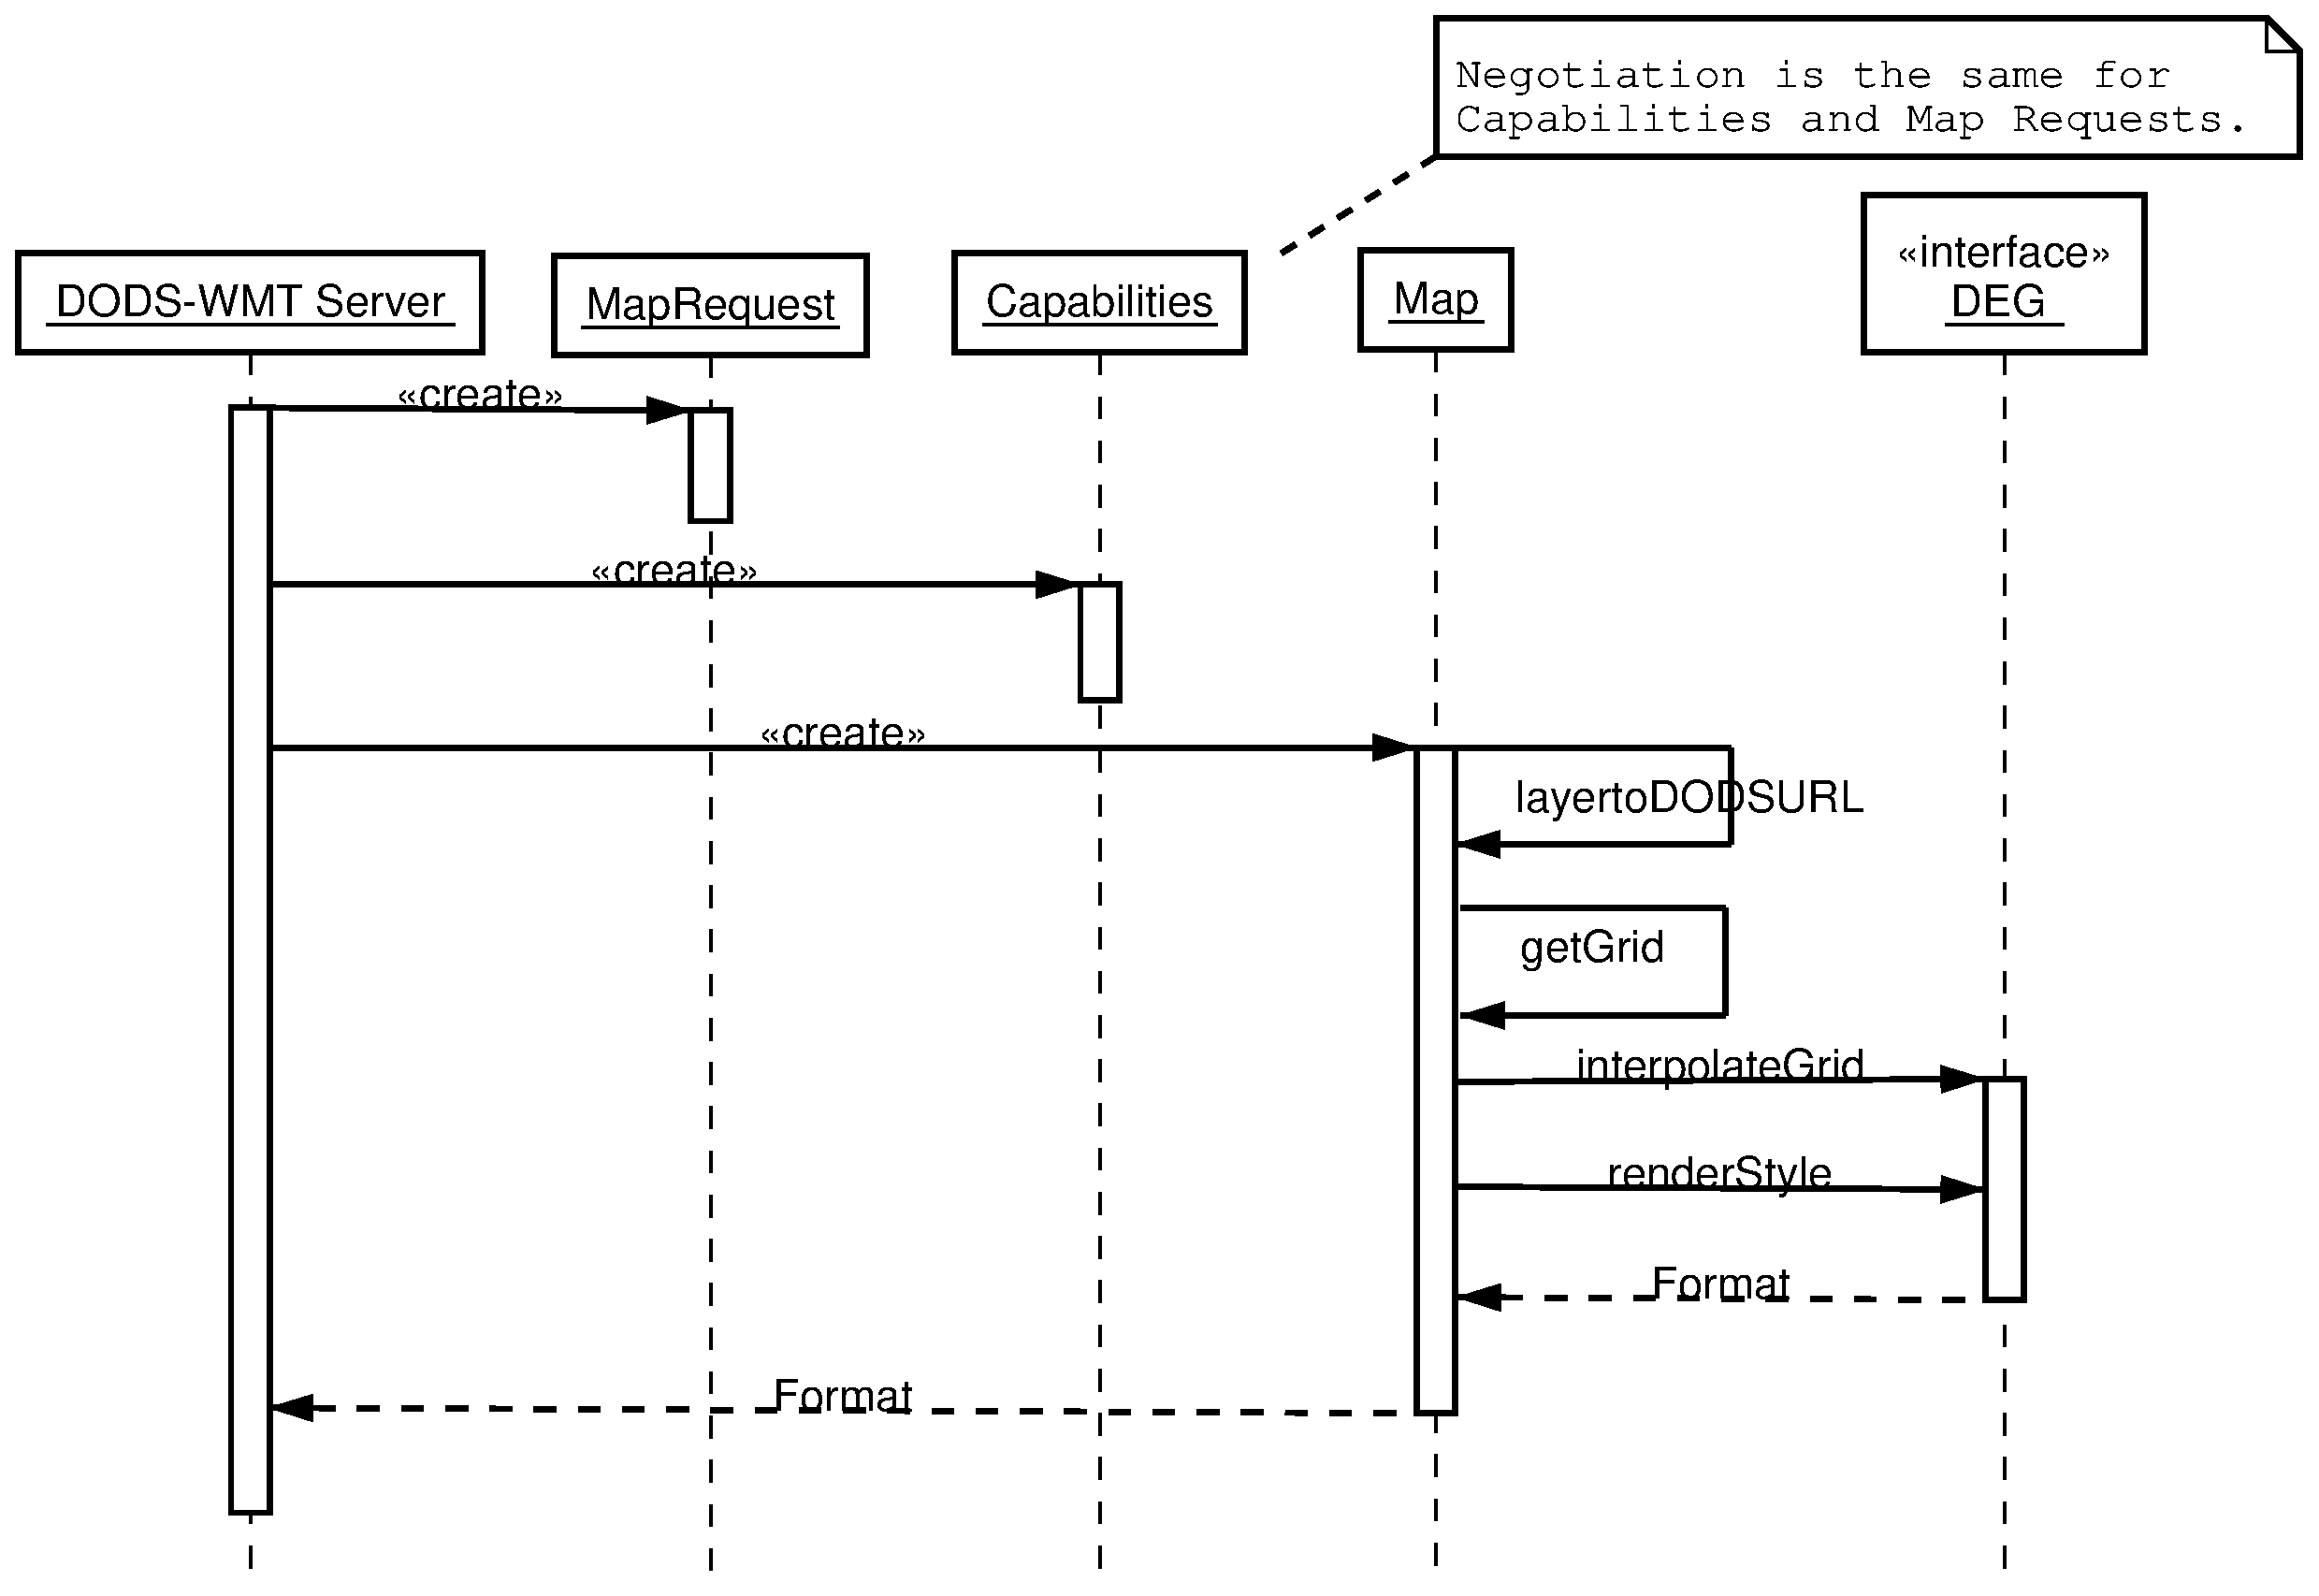
\epsfig{file=wmt-interaction-map.eps,width=8in}
% \caption{A sequence diagram for GetMap.}
% \label{fig:interacton-map}
% \end{center}
% \end{sidewaysfigure}

The Map object is the work horse of the DODS-WMT Gateway. It receives request
parameters from the MapRequest and information about the DODS-WMT
Gateway from the Capabilities object and, based on those parameters,
produces a picture of a map which is returned to the client (see section
[6.2.8.1]).

The Map object will return error information as per section [6.2.8.2.8] of
the WMT specification. Exceptions will be handled here instead of by a
separate object so that the Map may make use of the Render interface to
handle the INIMAGE exception value.

Unless an error is detected and an Exception is returned, the DODS-WMT
Gateway object will generate a valid HTTP response which contains the map
picture with a correct MIME header. If an error is detected, the DODS-WMT
Gateway object will return an error using XML if that is allowed given the
Exceptions parameter. If the Map object detected the error and generated a
message returned in a picture, the DODS-WMT Gateway object will return that.
See sections [6.2.8.3] and [6.2.8.4] of the WMT specification.

% Also note that the GSCF\_DEG
% class implements the DEG (Display Element Generator) interface and the Map
% class depends on that implementation to perform its tasks.

% Figure~\ref{fig:interacton-map} shows the objects involved in responding to a
% Map request.

\subsubsection{The DEG interface}
The DEG interface is the point where the work on this software to be carried
out by GSFC and DAS are tied together\footnote{In our implementation, we
  (DAS) have supplied two implementations of the DEG interface: A colorfill
  and default DEG.}. In this design we specify in the
simplest terms what this interface is to do, not how it is to be done. Some
of the possible implementations of the interface could include running filter
programs which read and write to and from standard input and output,
file-based processing, methods which use analysis tools such as IDL, etc.

A Map object may have several instances of DEG. This accommodates the WMT
specification's requirement that a WMT server support responses which combine
several layer/style instances. Each instance of DEG serves as a (smart)
container for a single layer/style.

\subsubsection{DodsURL}
\label{dodsurl}

The Class DodsURL is used to map a particular Layer named in the Capabilities
document to a DODS URL. This information is stored in the DataURL tag of the
Capabilities XML document.

A subclass of DodsURL included in the software is CatalogURL. This class
addresses making WMT requests of data sets which contain many possible data
sources. For example, the sample Capabilities XML document we include in the
software, uriavhrr.xml, provides access to a satellite data archive which
contains about 25,000 individual passes. The CatalogURL object provides a
way, using the Vendor Specific Parameters, to select a single pass from that
collection of aproximately 25,000.

The DEG interface uses DodsURL and/or CatalogURL to access the DODS URL for a
particular Layer named in the Capabilites XML/object.

\subsubsection{Layer}

A Layer object is the point int he WMT gateway where a DODS server is
contacted and data are read. The Layer object uses a URL passwd to it by the
DEG interface instance and dereferences that URL to access data. The data are
held by the Layer object in either an instance of DODS' Grid or Array class.
Layer provides methods which can be used to access these objects.

\subsubsection{SRS}

The SRS class specifies the interface for all SRS mapping operations
available within the WMT 1.0.0 specification. In practice this means mapping
a request given interms of a bounding-box to a DODS constraint expression
(CE) derived for a particular dataset (aka Layer). Thus one task the SRS
interface must perform is creation of the contraint information which,
combined with the DataURL returned by the DodsURL class, forms the complete
URL used by an instance of Layer to request information from a DODS data
server. 

The SRS interpolate() method is responsibe for taking a DODS Grid variable
and interpolating it to match the SRS and BBox. See section [6.2.8.2.2] and
[6.2.8.2.3] of the WMT specification.

Because the SRS interface maps the bounding-box to a DODS CE, the WMT Gateway
can make full use of DODS' constraint-based access features to limit the
amount of information read and transferred to only that information needed.

\subsubsection{Format}

The Format interface's output\footnote{The specific Style and Format
  information should be extracted from the MapRequest object which will be
  passed to renderStyle().} method is responsible for taking the DODS Grid
object and producing the corresponding map picture in the requested Format,
subject to the Style, Height, Width, Transparent and BGColor parameters of
the MapRequest.  See sections [6.2.8.2.4], [6.2.8.2.5], [6.2.8.2.6] and
[6.2.8.2.7].

The Format interface defines how a rendering engine is used generate one of
the output styles given DODS data. The Format class defiens an object that
can hold multiple DODS Grid or Array objects (delivered by instances of DEG).
The instance of Format, once it is loadded with DODS Grid or Array objects,
generates the requested output format. 

The instance of Format writes the output directly to standard output, which
the object assumes is the httpd's socket connected back to the requesting
process. 

\subsection{The FeatureInfo request}
This option item will not be implemented by this design unless there's extra
time to do so. See section [6.2.9].

\clearpage
\appendix

\section{Mapping of Requirements from the WMT Specification}
\begin{table}[h]
\caption{A mapping of the normative requirements listed in the WMT
  specification to design entities in this paper.}
\label{tab:requirements}
\vspace{12pt}
\begin{minipage}{\linewidth}
\begin{center}
\begin{tabular} {|ll|} \hline
\sc{Requirement} & \sc{Entity} \\ \hline
6.1.1 & Capabilities object \\
6.1.2 & Capability document \\ 
6.1.3 & DODS-WMT Gateway object \\
6.1.4 & Capabilities object \\ \hline
6.2.5 & MapRequest object \\ \hline
6.2.6 & NA\footnote{This requirement applies to clients} \\ \hline
6.2.7 & Capabilities object \\ \hline
6.2.8.1 & Map object \\
6.2.8.2.1 & Map object \\
6.2.8.2.2 & SRS Interface \\
6.2.8.2.3 & SRS Interface \\
6.2.8.2.4 & Format interface \\
6.2.8.2.5 & Format Interface \\
6.2.8.2.6 & Format Interface \\
6.2.8.2.7 & Format Interface \\
6.2.8.2.8 & Map object \\
6.2.8.3 & DODS-WMT Gateway object \\
6.2.8.4 & Map object \\ \hline
6.2.9 & NA\footnote{This requirement applies to FeatureInfo which is optional
  and not supported by the DODS-WMT Gateway}\\ \hline
\end{tabular}
\end{center}
\end{minipage}
\end{table}

\section{Revision history}
\begin{vcode}

$Log: wmt.tex,v $
Revision 1.12  2000/10/23 18:22:24  jimg
Updated to the delivered implementation.

Revision 1.11  2000/06/21 02:00:47  jimg
Fixed spelling/grammar errors.

Revision 1.10  2000/06/21 01:56:17  jimg
Added revision log.


\end{vcode}

\end{document}
